\chapter[Tuned Amplifier using IFT]{Tuned Amplifier using IFT}
\label{iftamplifier}
%-------------------
\section*{Aim}
To design and implement a tuned frequency amplifier using BJT and IFT.
%--------------------
\section*{Theory}


Intermediate frequency amplifiers are tuned voltage amplifiers used to amplify a particular frequency. Its primary function is to amplify only the tuned frequency with maximum gain and reject all other frequencies above and below this frequency. This type of amplifiers are widely used in intermediate frequency amplifiers in AM super heterodyne receivers, where intermediate frequency is usually 455 kHz.

In common emitter voltage amplifier circuit (emitter bypassed), the voltage gain is $A_V=\frac{R_C||R_L}{r_e}$, where $R_C$ is the collector resistance in the circuit, $R_L$ is the load resistance and $r_e$ is the internal emitter resistance. In tuned voltage amplifier the collector resistance is replace by a tuned load upon which  the gain is dependant. For a parallel resonating circuit cosisting of a capacitor, C and an inductor,L the impedance $Z_o$ is maximum at resonant frequency, $f_o=\frac{1}{2\pi \sqrt{LC}}$. So an amplifier with tuned load will have maximum gain at resonant frequency.
In practical tuned amplifier circuits, an intermediate frequency transformer(IFT) is used as tuned load. IFT is tuned to standard 455 kHz audio frequency, (See \ref{IFT}).

The quality factor of the circuit is given by $Q=\frac{f_o}{Bandwidth}$.

\section*{Design}
Inorder to design a common emitter amplifier operating at high frequency, one can use a high frequency transistor like BF194, BF195, BF494, BF495 or 2N2222.
\\Choose transistor BF 194/195. For its datasheet See \ref{BF194/195},\\


\noindent Let $V_{CC}$ be 10\% more than the required output amplitude, ie. 10V.
\begin{equation}
\therefore V_{CC}=12\ V
\end{equation}
\begin{equation}
I_c<10 \% \ of \  I_{Cmax} =\ 10\%\  of\  30\  mA =\ 3 mA
\end{equation}
\noindent Let $I_c=\ 1 mA$.
%\noindent The current gain,
%\begin{equation}
%h_{FEmin}=\ 67
%\end{equation}
Let the stability factor of the circuit be,
\begin{equation}
S=10
\end{equation}

\noindent Under dc  conditions, the primary dc resistance of the IFT is very small($<5\Omega$). So dc voltage drop across collector circuit is very low, approximately zero.

\noindent For class A mode of operation set, 
\begin{equation}
 V_{CE} = \frac{V_{CC}}{2}= 6 V
\end{equation}
\paragraph{Design of Emitter resistance}
\noindent \\The voltage across emitter resistance is,
\begin{equation}
V_{RE}=V_{CC}- V_{CE} =\ 12V-\ 6V=\ 6V
\end{equation}
\begin{equation}
I_E \approx I_C 
 \end{equation}
\noindent Hence
\begin{equation}
I_E = 1mA
\end{equation}
\noindent Thus
\begin{equation}
R_E=\ \frac{V_{RE}}{I_E}=\ \frac{6V}{1mA}=\ 6k\Omega
\end{equation}
\noindent Choose standard value of $R_E=\ 5.6 \ k\Omega$.
\paragraph{Design of Potential divider biasing\\}
\noindent The Stability factor S=10. Assuming $R_B$ is the effective resistance at the base,
\begin{equation}
S=\ 10=\ 1+\frac{R_B}{R_E}
\end{equation}
\begin{equation}
R_B=\ 9R_E=\ 50.4k\Omega
\end{equation}
\begin{equation}
\label{R1R2}
R_B=\ R_1||R_2=\ \frac{R_1R_2}{R_1+R_2}=\ 50.4k\Omega
\end{equation}
\noindent The voltage at the base of the transistor is 
\begin{equation}
V_B=\ V_E+\ V_{BE}=\ V_{RE}+\ V_{BE}=\ 6V+\ 0.6V=\ 6.6 V
\end{equation}

\noindent This is the voltage across $R_1$. 
\begin{equation}
V_{R1}= V_{CC} \frac{R_2}{R_1+R_2}=\ 6.6V
\end{equation}

\begin{equation}
\label{R2}
\frac{R_2}{R_1+R_2}=\ \frac{6.6V}{12V}=\ 0.55
\end{equation}
From equations \ref{R1R2} and \ref{R2}, 
\begin{equation}
R_1=\ 91.4\ k\Omega \approx \ 82\ k\Omega \ and \ R_2=100\ k\Omega
\end{equation}
\noindent Choose load resistor as 
\begin{equation}
R_L=\ 100 k\Omega
\end{equation}
\subsubsection{Design of capacitors}
\noindent The capacitors $C_1$, $C_2$  and $C_E$  can be designed based on lower cut-off frequency at -3 dB point. Since this frequency is much lower than 300 kHz, Choose low values of capacitance like \begin{equation}
C_1=\ C_2=\ C_E=\ 1 \ \mu F
\end{equation}

\section*{Circuit Diagram}
See Figure \ref{IFTuned} for circuit diagram.
\begin{figure}[ht]
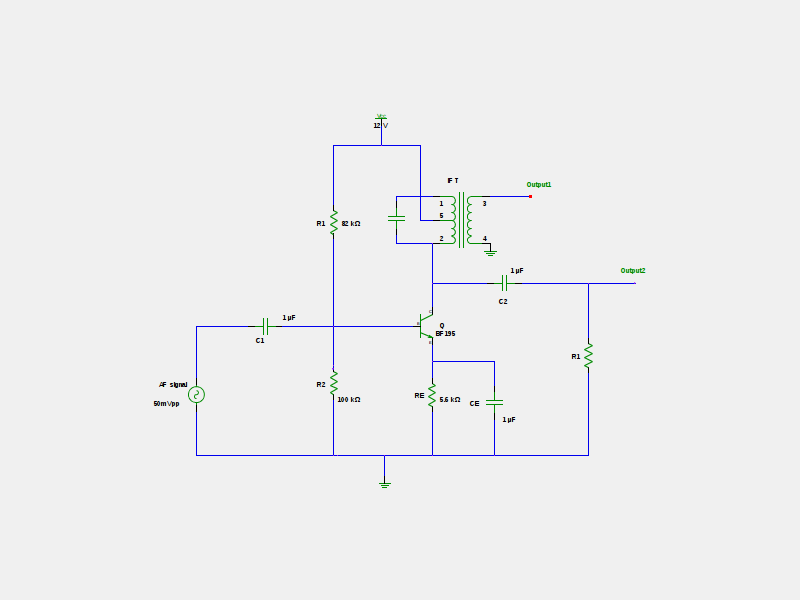
\includegraphics[width=12cm, height=8cm, trim=2cm 3.5cm 5cm 3.5cm,clip=true]{IFTuned.png}
\caption{Circuit Diagram for IF Tuned Amplifier}
\label{IFTuned}
\end{figure}
\section*{Procedure}
\begin{itemize}
\item
Assemble the circuit as shown in the circuit diagram.
\item
Obtain output from output-1 or output-2 terminal as in the circuit diagram.
\item
Give input signal, which is a sinewave of frequency variable from 300 kHz to 600 kHz and amplitude 50 $mV_{pp}$.
\item
Observe the output waveform on a CRO. 
\item
Enter the details of input and output waveforms on the tabular column shown.
\item
Calculate gain $A_V$ by varying $f_{in}$.($A_V= \ \frac{V_{outpp}}{V_{inpp}}$)

\item
Plot frequency response characteristics with $f_{in} (kHz) $ along x-axis and  $Gain_{dB}=\ 20\ log\ A_v$ along y-axis.
\item
Find the resonant frequency, 3-dB bandwidth and hence the Q-factor.
\end{itemize}
\section*{Observation}
\begin{center}

\begin{tabular}{|l|l|l|l|l|}

\hline
  & & & &\\
 
$f_{in} (kHz) $  & $log_{10}\ f_{in}$  &  $V_{outpp}(V)$ & $A_v\ =\frac{V_{outpp}}{V_{inpp}} $ & $Gain_{dB}=\ 20\ log\ A_v$ \\ \hline
 & & & &\\ \hline
& & & &\\ \hline
& & & &\\ \hline
& & & &\\ \hline
& & & &\\ \hline
& & & &\\ \hline

\end{tabular}
\end{center}
%\textcolor{red}{TODO:frequency response curve of gain to be added}. 
\section*{Result}
A tuned amplifier was implemented using IFT.\\
Its maximum gain= \\
Resonant frequency= \\
Band-width=\\
Q-factor= 
